
%% bare_jrnl.tex
%% V1.4b
%% 2015/08/26
%% by Michael Shell
%% see http://www.michaelshell.org/
%% fores IEEEtran.cls version 1.8b or later) with an IEEE
%% journar current contact information.
%%
%% This is a skeleton file demonstrating the use of IEEEtran.cls
%% (requil paper.
%%
%% Support sites:
%% http://www.michaelshell.org/tex/ieeetran/
%% http://www.ctan.org/pkg/ieeetran
%% and
%% http://www.ieee.org/

%%*************************************************************************
%% Legal Notice:
%% This code is offered as-is without any warranty either expressed or
%% implied; without even the implied warranty of MERCHANTABILITY or
%% FITNESS FOR A PARTICULAR PURPOSE! 
%% User assumes all risk.
%% In no event shall the IEEE or any contributor to this code be liable for
%% any damages or losses, including, but not limited to, incidental,
%% consequential, or any other damages, resulting from the use or misuse
%% of any information contained here.
%%
%% All comments are the opinions of their respective authors and are not
%% necessarily endorsed by the IEEE.
%%
%% This work is distributed under the LaTeX Project Public License (LPPL)
%% ( http://www.latex-project.org/ ) version 1.3, and may be freely used,
%% distributed and modified. A copy of the LPPL, version 1.3, is included
%% in the base LaTeX documentation of all distributions of LaTeX released
%% 2003/12/01 or later.
%% Retain all contribution notices and credits.
%% ** Modified files should be clearly indicated as such, including  **
%% ** renaming them and changing author support contact information. **
%%*************************************************************************


% *** Authors should verify (and, if needed, correct) their LaTeX system  ***
% *** with the testflow diagnostic prior to trusting their LaTeX platform ***
% *** with production work. The IEEE's font choices and paper sizes can   ***
% *** trigger bugs that do not appear when using other class files.       ***                          ***
% The testflow support page is at:
% http://www.michaelshell.org/tex/testflow/



\documentclass[journal]{IEEEtran}


% correct bad hyphenation here
\hyphenation{op-tical net-works semi-conduc-tor}

\usepackage{graphicx}
\usepackage{caption}
\usepackage{hyperref} 
\usepackage{xcolor}

\hypersetup{
    colorlinks,%replace ugly boxes by simply coloring hyperlinks, using following settings
    linkcolor={red!60!black},
    citecolor={green!50!black},
    urlcolor={blue!80!black}
}

\begin{document}

\title{INF6600 Rapport TP4 \\ Améliorations au système de contrôle d'un drone fermier}


\author{Daniel~Lussier-Lévesque et Ian~Gagnon}

\maketitle

\begin{abstract}
L'implémentation d'un système de contrôle de drone fermier a été réalisé progressivement tout au long de la session en commençant par un module TrueTime avec un système continu déjà implémenté en Simulink. Par la suite, l'implémentation a continué sur une machine virtuelle QNX roulant sous VMware, avec certaines fonctions déjà fournies. Ce rapport se concentre sur ce qui a été fait sur cette base de code pour améliorer les aspects les plus importants. La première étape a été d'implémenter un système de log qui nous permettent de voir comment se comporte l'ordonnancement des tâches et la performance du système. Par la suite, malgré le manque de droits d'accès qui nous permettraient de comprendre l'ensemble des problèmes de performance, nous avons toutefois été capable de les mesurer et de les documenter. Un système graphique vivant en dehors de la machine virtuelle nous permettant de valider le comportement du système a aussi été implémenté.
\end{abstract}


\section{Introduction}
\IEEEPARstart{L}{e} système de contrôle considéré est celui d'un drone autonome capable de se déplacer sur trois axes et ayant une caméra fixe pour prendre en photo l'ensemble d'un champs. Le drone doit naviguer les champs et prendre des photos jusqu'à ce que la mémoire soit pleine, puis transmettre les photos à une station base. Lorsque la batterie est presque vide (10\%), le drone doit retourner à la station base pour être rechargé. 

Le système de contrôle implémente le contrôle de la navigation (où le drone va), le contrôle de la batterie (est-il temps d'aller recharger la batterie?) et le contrôle mission (quelle séquence d'étapes doit être exécutée pour opérer avec succès?).

Le système de contrôle de drone sur lequel nous avons apportés nos modifications est un système simple où la communication entre le système continu et discret est effectué par des variables atomiques et par l'enregistrement de \textit{callbacks}. La communication en dehors du système s'effectue par des messages de log sur la console de debug où à intervalle régulier (chaque seconde) l'état du drone est envoyé. Toutes les tâches sont asynchrones les unes par rapport aux autres et roulent sur leur propre fil d'exécution. Nous avons choisi de mettre à jour le système de contrôle du drone toutes les 100 ms.

De plus, l'implémentation du système de contrôle doit être accompagné d'une plateforme de simulation d'un environnement dans lequel opérer, qui comprend le temps de réponse de la caméra, les variations d'orientation et de vitesses, le temps de transmission de photo à la station base et la charge et décharge de la batterie. Le système continu est mis à jour toutes les 20ms de sorte qu'il soit significativement plus rapide que le système de contrôle. De cette manière, le système discret ne voit pas énormément de différence dépendamment s'il se fait juste avant ou juste après une mise-à-jour du système continu.

L'ensemble des photos prises peut être visualisé à travers une carte de la ferme qui est mise à jour à chaque transmission et montre quelle région a été prise en photo. La carte doit être accédée en allant chercher les fichiers sur le système de fichier de la machine virtuelle.

La politique d'ordonnancement utilisée est un systèmes de priorités fixes et un ordonnancement FIFO pour chaque niveau de priorité. Le choix a été fait de placer la priorité du contrôle caméra avant celle du contrôleur de navigation parce qu'il est plus facile de compenser pour une échéance manquée dans le cas de la navigation (une photo manquée implique de défaire les dernières mise-à-jour de navigation pour reprendre la photo).

La machine virtuelle roule sous QNX 7.0 sous VMware Workstation avec un hôte Windows 10. La machine hôte à un processeur d'Intel à quatre coeurs, le i7 3770, avec 16 GB de mémoire DDR3 et utilise un Seagate ST1000DM003 comme disque dur. 


\section{Lacunes du système de base}
\label{lacunes}

Le système décrit plus haut a plusieurs lacunes importantes. Nous allons ici nous focaliser sur les trois principales faiblesses qui nous ont empêcher de réaliser correctement plusieurs améliorations auxquels nous avions pensés. Il va s'en dire que nous avons penser plus important de régler ces lacunes au meilleur de nos capacités en priorité.

\subsection{Peu de visibilité sur l'état du système et sur la qualité de l'ordonnancement}

Le principal problème est qu'avec le système de base, nous ne savons pas si le système est \emph{correct}, c'est à dire que le système effectue les actions que l'ont s'attend à ce qu'il fasse. Les messages de logs qui sont envoyés sont répétitifs et il est facile de manquer un comportement anormal dans les 1800 messages que comportent une séquence d'exécution. De plus, il est impossible de savoir ce qui se passe à l'intérieur de cette période d'une seconde. Une période plus courte n'est toutefois pas envisageable: il serait impossible d'analyser l'entièreté des messages en temps réel et donc encore plus facile de manquer une information inattendue. Il n'est pas non plus envisageable d'analyser les données à la fin de la simulation: la console de debug ne peut contenir qu'un nombre limité de messages.

En conséquence, il n'est pas possible de qualifier le système d'aucune manière: un problème de comportement du système demanderait une correction importante au code qui invaliderait l'ensemble des mesures effectuées. Comme une séance de simulation dure 20 minutes, il serait difficile d'arriver à un ensemble de résultats suffisant dans un temps raisonnable si nos mesures devaient être invalidés. Sans mesures fiables, il est impossible de déterminer si une tentative d'amélioration du système améliore réellement le système.

En assumant que le comportement du système est correct, nous ne pouvons toujours pas penser à améliorer les performances du système ou rajouter de nouvelles fonctions utiles parce que nous n'avons aucune métrique de performance de disponible. Nous ne savons pas si les tâches manquent leur échéance de manière régulière et arrivent tout juste à rester fonctionnels, ou au contraire si il y a largement de ressources disponibles pour de nouvelles tâches.

Dans le cas où le comportement du système n'est pas celui attendu, les métriques de qualité d'exécution nous sont aussi utile pour comprendre les problèmes. Si une tâche est en famine parce que les tâches plus prioritaires prennent toutes les ressources, ce sera facilement visible et évitera une longue séance de debug en aveugle.

\subsection{Pics de latence}

Après avoir apportées les modifications qui seront détaillées à la section \ref{ameliorations}, nous avons réalisé que le système tel que simulé avait encore une lacune qui bloquait des améliorations que nous avions planifiés: le système est affecté par des pics de latence non-déterministes. Ces pics de latences affectent toutes les tâches en même temps. Plus spécifiquement, ils affectent des tâches qui n'acquirent pas de mutex où autre verrou global et communiquent uniquement par des variables atomiques. On peut donc supposer que ces pics arrivent au niveau système et non au niveau de l'ordonnancement ou au niveau de la communication. 

En plus d'affecter les performances du systèmes et de le rendre moins fiable, un impact important de ces pics de latences est que toutes les métriques de pire temps d'exécution ou de déviations standard sont affectées de manière aléatoire et qu'une comparaison avant et après une tentative d'amélioration est noyée dans le bruit de ces pics.

Les pics des latence durent plusieurs millisecondes. Plusieurs tentatives de contourner le problème ont été essayé: réduire le nombre de cœurs du système de contrôle, augmenter le nombre de cœurs du système et déplacer la machine virtuelle du disque réseau au disque dur local. Déplacer la machine virtuelle à permis de réduire significativement la durée de ces pics, mais aucune des ces tentatives n'a permis de ramener les variations de latences à des temps raisonnables.

\section{Améliorations apportées}
\label{ameliorations}

\begin{figure}
	\centering
	\captionsetup{justification=centering}
	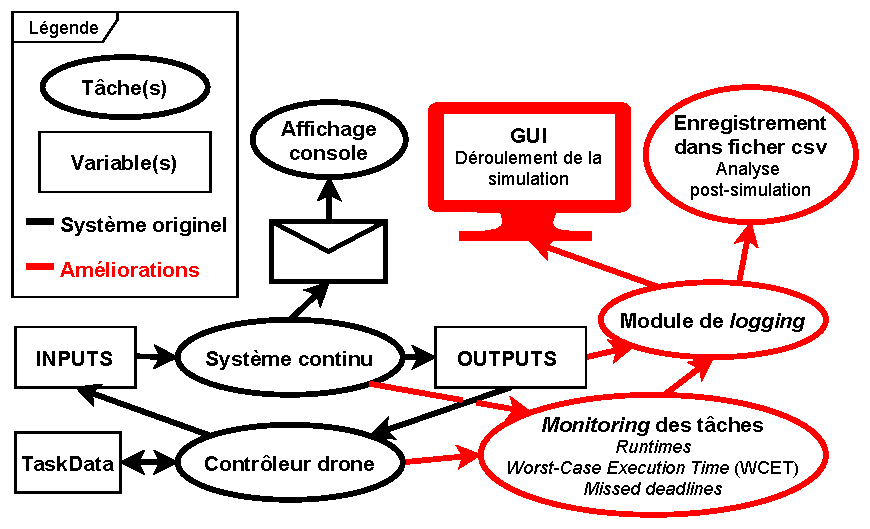
\includegraphics[width=\linewidth]{diagrammeDeTaches_Simple.pdf}
	\caption{Diagramme de tâches du système}
	\label{taskDiagram}
\end{figure}

Pour remédier aux lacunes présentées à la section précédente, des améliorations sont proposées et illustrées à la Figure \ref{taskDiagram}. Un \textit{monitoring} des tâches récolte d'abord les métriques d'exécution pour chaque tâche, un module de \textit{logging} sert ensuite à regrouper les informations pour finalement les enregistrer en format csv. En supplément, un \textit{Graphical User Interface} (GUI) permet de suivre le déroulement de la simulation en temps réel.

\subsection{Monitoring des tâches}

Pour chaque tâche qui s'exécute, le temps d'exécution est calculé en faisant la différence entre les temps initiaux et finaux obtenus par la fonction \verb|std::chrono::steady_clock::now()| et enregistrés dans des variables atomiques. Ainsi, la durée de la dernière exécution (\textit{last runtime}), le pire cas (WCET ou \textit{Worst-Case Execution Time}) et les échéances manquées sont comptabilisés. L'horloge du système, avec sa granularité d'une milliseconde, limite la précision des données.

\subsection{Logging}

Une fois que nous avons implémenté le code pour avoir l'information dans des variables, il faut penser à un moyen de la communiquer. Il a donc fallu implémenter une nouvelle fonction (avec le code de \textit{monitoring} associé) pour lire l'ensemble des variable et les transmettre vers les nouvelles sorties. Nous avons décider d'exécuter la tâche toutes les 100 millisecondes afin de ne pas surcharger le système. Cette fonction est appelée par la tâche de \textit{monitoring} déjà existante qui auparavant ne poussait les donnée que vers la console une fois toute les secondes.

\subsection{Sortie en fichier csv}

La sortie qui permet de faire une analyse compréhensive du système est un simple fichier csv qui est sauvegardé en mémoire non-volatile au fur et à mesure que la simulation avance. Le format csv étant supporté par pratiquement tous les outils d'analyse et de base de données, il est donc facile de s'en servir pour obtenir des statistiques sur un grand nombre d'exécutions pour ensuite les formater adéquatement en tableaux, en graphiques ou en générant un rapport. En effet, que ce soit à l'aide de langages de scripts (Python, R ou MATLAB) ou à l'aide d'un tableur (Microsoft Excel ou LibreOffice Calc), l'analyse sera infiniment plus poussée que celle obtenue avec la sortie en console.
 
\subsection{GUI}
Un GUI a été implémenté en Python afin de suivre l'avancement de la simulation. Comme il s'agit d'une preuve de concept et que le focus de ce projet est l'implémentation sous QNX, l'interface graphique est limitée à un strict minimum (voir section~\nameref{resultats}). L'accent est plutôt mis sur le transfert de données. À cet égard, l'hypothèse (très réaliste) que le drone transmet ces images à la base via une connexion réseau est émise et cette connexion est exploitée pour établir la communication avec le GUI en utilisant un \textit{socket} avec le protocole TCP/IP. Une convention doit être choisie afin d'assurer un bon transfert de données: message d'une longueur fixe, message délimité (i.e. avec caractères spéciaux de début et fin) ou  message avec une entête indiquant sa longueur. Ici, pour garder le tout le plus simple possible, la longueur des paquets est fixée et des caractères de remplissage (i.e. des espaces) sont ajoutés à la fin des trames de données pour ajuster la taille des paquets. De plus, un délai sur la connexion, une gestion de déconnexion ainsi qu'un avertissement de fin de simulation sont ajoutés pour prévenir les erreurs et éviter les \textit{deadlocks}.

\section{Résultats}\label{resultats}

\subsection{Analyse du système}
Avant d'analyser le système en détails à l'aide du fichier csv fournit par nos améliorations, la fonctionnalité de l'implémentation de base est validée à la l'aide de l'image en sortie de la simulation générée par la fonction \textit{transmitPhotos()}. L'image recadrée (Figure \ref{fig:farmMap}) démontre effectivement que l'intégralité du champ 22, soit le champ balayé lors de la simulation, a été photographié.

\begin{figure}
	\centering
	\captionsetup{justification=centering}
	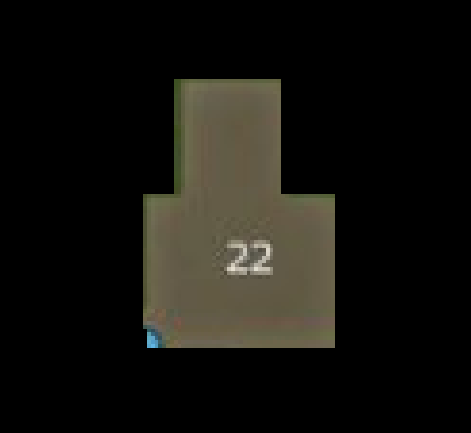
\includegraphics[width=0.7in]{farmMap.png}
	\caption{Image agrandie de la zone couverte par le drone}
	\label{fig:farmMap}
\end{figure}

L'analyse du système est réalisée en deux parties. D'une part, le comportement du système est examiné pour valider que celui-ci fait bien ce qu'il doit faire et ce sans écart de conduite (i.e. comportement anormal). Pour illustrer la conformité de notre système en simulation, nous avons décidé de tracer les courbes des variables d'état (vitesses, orientation, batterie, mémoire, etc). De cette manière, nous pouvons aisément comparer nos résultats avec les courbes obtenues de la simulation sous TrueTime générées à une étape précédente de ce projet. Les résultats concordent dans l'ensemble, sauf quelques écarts attribuables aux différences entre les systèmes continus (e.g. le temps de recharge). Un exemple est donné à la Figure \ref{fig:comparaisonVh} où les vitesses horizontales pour les deux simulations sont comparées. On remarque que l'allure des courbes est bel et bien similaire. Une vue agrandie de la courbe de QNX permet d'apprécier les détails du pas de temps rapproché qui permet de qualifier les régimes transitoires, dans ce cas, comment un changement d'orientation et de consigne de vitesse affecte la vitesse horizontale réelle, ce qui était impossible avec les données sorties sur la console.

\begin{figure}
	\centering
	\captionsetup{justification=centering}
	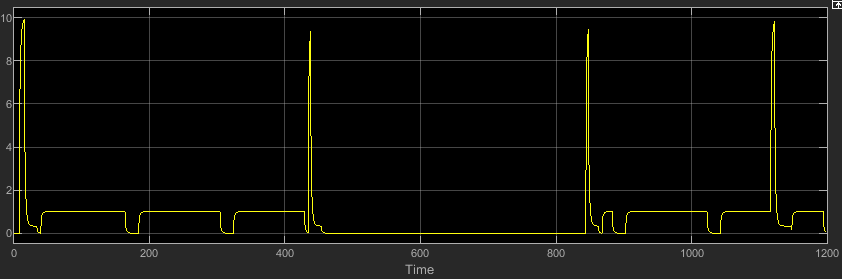
\includegraphics[width=2.8in]{TrueTimeVh.png}
	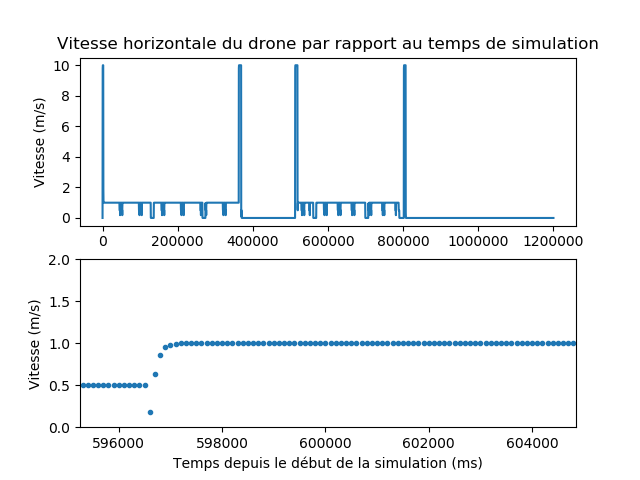
\includegraphics[width=\linewidth]{csv_variable_etat.png}
	\caption{Comparaison de la vitesse horizontale obtenue sous TrueTime (noir) et QNX (blanc)}
	\label{fig:comparaisonVh}
\end{figure}

D'autre part, la qualité de l'ordonnancement est étudiée à l'aide du \textit{Worst-Case Execution Time} (WCET), une métrique populaire dans l'étude des systèmes temps réel. Pour ce faire, trois tâches périodiques (orientation, vitesse et batterie) sont analysées graphiquement à deux reprises. Les résultats sont présentés à la Figure \ref{fig:perfoTrois}. On constate que les pires temps d'exécution varient entre les tâches, au cours de la simulation et entre les essais. La variation entre les tâches est justifiable puisque différentes tâches prennent différents temps pour s'exécuter. La variation qui survient durant la simulation est explicable par le fait qu'une tâche puisse être préemptée par d'autres tâches plus prioritaires, rallongeant ainsi son exécution en fonction de la coordination des tâches au fil de la simulation. Cependant, sachant qu'il s'agit de la même simulation qui est roulée plusieurs fois sur la même machine dans les mêmes conditions, les performances d'ordonnancement ne devraient pas varier avec les essais. En d'autres termes, les résultats devraient rester constants entre deux simulations. Pour corroborer ce résultat intriguant, nous avons refait trois essais avec la tâche qui semblait la moins stable en terme de WCET, soit l'orientation. Le résultat (Figure \ref{fig:perfoOrientation}) confirme nos craintes: il survient des pics de latence non-déterministes dont l'origine est inconnue. Des analyses plus approfondies seraient nécessaires pour en déterminer la cause. Nous pensons qu'il s'agit d'un accès disque bloquant (l'ordre de grandeur serait le bon) soit du côté du système hôte (MS Windows) ou de la machine virtuelle (QNX), mais sans droit d'utilisateurs élevés il ne nous est pas possible de faire les tests qui pourraient le confirmer.

\begin{figure}
	\centering
	\captionsetup{justification=centering}
	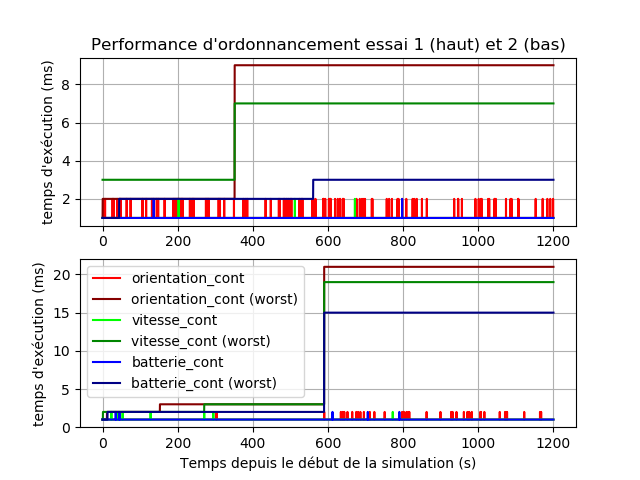
\includegraphics[width=220pt]{csv_try_1_2.png}
	\caption{WCET pour trois tâches avec deux essais}
	\label{fig:perfoTrois}
\end{figure}

\begin{figure}
	\centering
	\captionsetup{justification=centering}
	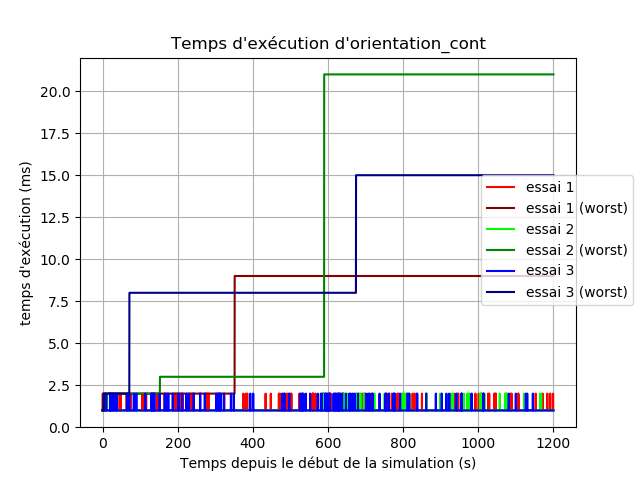
\includegraphics[width=200pt]{orientation_cont.png}
	\caption{WCET pour l'orientation avec trois essais}
	\label{fig:perfoOrientation}
\end{figure}

\subsection{Description du GUI}

\begin{figure}
	\centering
	\captionsetup{justification=centering}
	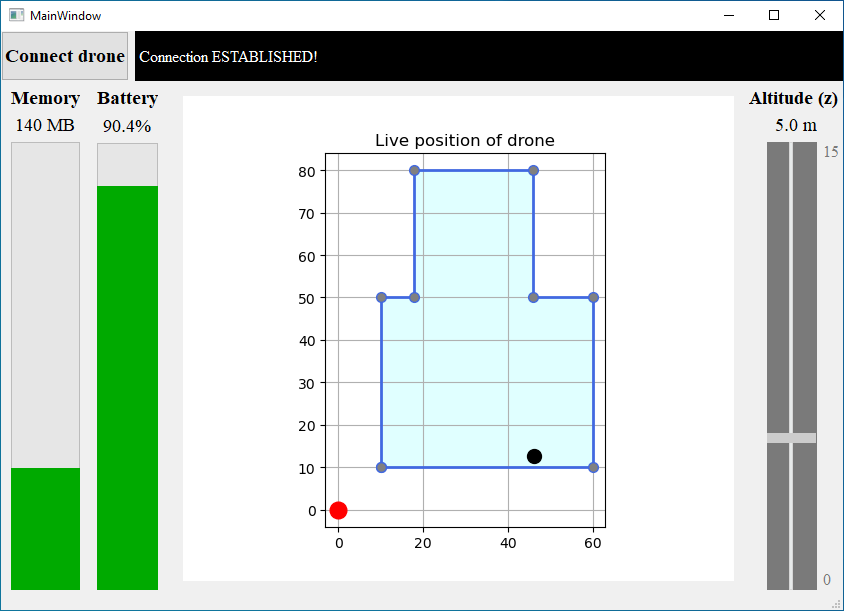
\includegraphics[width=200pt]{GUI_image.png}
	\caption{GUI durant la simulation}
	\label{fig:GUI}
\end{figure}

Dans la communication TCP/IP, le serveur roule sur QNX et le client sur le GUI. Après avoir ouvert le GUI, il faut donc d'abord lancer la simulation QNX (qui va partir le serveur) et ensuite appuyer sur le bouton "Connect drone" pour établir la connexion. Le GUI, présenté à la Figure \ref{fig:GUI}, affiche les paramètres de base de la simulation, soit: la mémoire, le niveau de batterie, la position du drone (x, y) et son altitude (z). De plus, une vidéo montrant le GUI en fonction (i.e. la simulation en accélérée) est disponible: \href{https://drive.google.com/file/d/1W9yt0Z4YxCwr0TjXkgv12WVO9TSmWGtv/view?usp=sharing}{INF6600-GUI-DEMO}\cite{ref:video}.

\section{Conclusion}
Dans cet article, nous avons décrit les améliorations apportées à l'implémentation d'un système de contrôle de drone fermier. L'analyse du système de base a soulevé des lacunes importantes en ce qui concerne les visibilités de l'état du système et de la qualité de l'ordonnancement. En effet, ce manque d'informations rend l'analyse du système et de ses performances difficile, voire impossible. 

Afin de pallier à ce manque de données, nous avons dans un premier temps implémenté un \textit{monitoring} des tâches avec un module de \textit{logging} permettant de recueillir de précieuses informations et de les enregistrer pour les analyser ultérieurement. Cela nous a permis d'étudier le système et de réaliser que des pics de latence imprévisibles affectait le système.
L'ensemble du code du système de contrôle et les résultats de simulations sont disponibles sur un dépôt GitHub\cite{ref:code}.

Dans un second temps, nous avons ajouté un GUI communiquant avec le drone via une connexion réseau utilisant les protocoles TCP/IP. Ce dernier affiche l'état du système durant la simulation et aide l'utilisateur à repérer un comportement inattendu du drone. Dans l'optique d'un déploiement réel du système sur une ferme, cette interface graphique roulant au niveau de la base d'opérations s'avérerait utile puisqu'elle permettrait au fermier du suivre le drone lors de sa mission et de réagir en cas de problèmes.

Les travaux futurs s'attarderont premièrement à comprendre la source et éliminer les pics de latences. Il serait intéressant d'étudier le système avec la machine virtuelle roulant uniquement sur un disque dur virtuel en mémoire pour voir si la source se trouve au niveau des accès disques. La meilleure option serait de rouler le système sur du matériel dédié.

Deuxièmement, la sécurité du système pourrait être rehaussée par l'utilisation de partitions. En isolant les processus de cette manière, on éviterait que la défaillance d'une tâche fasse planter tout le système. Par exemple, une erreur du système de communication n'aurait aucun impact sur le système de navigation, ce qui n'est pas une certitude présentement.

Dernièrement, d'un point de vue sécurité pour une utilisation réelle du système, il serait pertinent d'ajouter un bouton d'urgence à l'interface graphique pour arrêter le drone de force ou le ramener immédiatement à la base dans le cas où l'algorithme de contrôle aurait un raté (e.g. un mauvais calcul qui enverrait le drone à 1000 m d'altitude). 


\begin{thebibliography}{1}

\bibitem{ref:video}
Ian Gagnon, Daniel Lussier-Lévesque, \emph{Demonstration du GUI pour drone},\newline
https://drive.google.com/file/d/\newline
1W9yt0Z4YxCwr0TjXkgv12WVO9TSmWGtv/view?usp=sharing.

\bibitem{ref:code}
Ian Gagnon, Daniel Lussier-Lévesque, \emph{INF6600},\newline
https://github.com/IanGagnon7/INF6600.


\end{thebibliography}


% that's all folks
\end{document}


